\chapter{Development of the FPGA Firmware for the SFH}\label{cha:development}
\section{Overview of the Firmware}

The firmware in this thesis was developed for only two of three Artix-7 FPGAs integrated into the iFTDC, as detailed in Section \ref{sec:iFTDC}.
The third FPGA was excluded due to the incomplete development of its Ethernet connection.
\newline
The firmware of the different FPGAs differs only by their port assignment but are otherwise identical.
\newline
The firmware must perform several functionalities.
\newline
The main tasks of the firmware are to configure the Citiroc1A ASICs, explained in Section \ref{sec:configuration},
 communicaton with the controlling coputer via ethernet and the IPBUS protocol and a provisional readout of the time triggerd data from the Citiroc1A ASICs.
\newline
The fimrmware is written in VHSIC Hardware Description Language (VHDL) and is synthesized and implemented using Xilinx Vivado.
Several IP-cores, provided by Xilinx, are used to simplfy the development of the firmware for several tasks like the implementation of the configuration memory.
\subsection{The IPBUS Protocol}
The IPBUS protocol used for the communication between the FPGA and the controlling computer is a simple protocol for controlling IP-aware hardware devices with a 32 bit read and write bus using UDP as the transport protocol.\autocite{IPBUS_article}
\newline
The IPBUS protocol defines a read and write command enabling successful write and read operations of a 32 bit register, with a 32 bit address in the FPGA.    
\newline
The commands can be issued on the controling computer with the $\mu$HAL library, which allowes the user to issue read and write commands using a python script and an XML file defining the addresses of the registers.\autocite{IPBUS_article}
\newline
The address space inside the FPGA is defined in the firmware. The address space is divided into seprate address spaces for each of the slaves by the leading bits of the address.
For some slaves, the address space is further divided into subspaces for the different registers of the slave.


\subsection{The Firmware Structure}
\begin{figure}[H]
    \centering
    
\begin{tikzpicture}[node distance=2cm]

    % Top-level module
    \node (top) [block] {Top-Level Module};
    
    % Submodules
    \node (wrapper) [block, below =1.5cm and 0.5cm of top] {Wrapper Module};
    \node (sync) [block, below left  =1.5 cm and 0.5cm of top] {Synchronizer Module};
    
    % Wrapper components
    \node (ipbus) [block, below left=1.5cm and 2.5cm of wrapper] {IPBBUS Protocol Logic};
    \node (addr) [block, below right =1.5cm   and 1.5cm of wrapper] {Address Decoding Logic};
    \node (slaves) [block, below =1.5cm and 1.5cm of wrapper] {Slave Module};
    
    
    % Slave module components
    \node(Citiroc1A 1)[block, below left=2cm and 0cm of slaves] {Citiroc1A ASIC 1};
    \node(Citiroc1A 2)[block, below right  =2cm and 0cm of slaves] {Citiroc1A ASIC 2};
    %ASIC 1
    \node (config1) [block, below left =1.5cm and 1cm of Citiroc1A 1 ] {Citiroc1A Interface};
    \node (hitcounters1) [ block, below  =1.5cm and -1.5cm of Citiroc1A 1] {Hit Counters (32)};
    %ASIC 2
    \node (config2) [block,  below right =1.5cm and -1cm of Citiroc1A 2] {Citiroc1A Interface};
    \node (hitcounters2) [ block,below left = 1.5cm and -1.5cm    of Citiroc1A 2] {Hit Counters (32)};
    %config1
    \node (confi1) [block, below =1.5cm and -1cm of config1 ] {Configuration SM};
    \node (verif1) [block, below right =1.5cm and 1cm of config1] {Verification SM};
    %config1
    \node (confi2) [block, below =1.5cm and -1cm of config2 ] {Configuration SM};
    \node (verif2) [block, below left  =1.5cm and 1cm of config2] {Verification SM};
    % Arrows
    \draw [arrow] (top) -- (wrapper);
    \draw [arrow] (top) -- (sync);
    \draw [arrow] (wrapper) -- (ipbus);
    \draw [arrow] (wrapper) -- (addr);
    \draw [arrow] (wrapper) -- (slaves);
    \draw [arrow] (slaves) -- (Citiroc1A 1);
    \draw [arrow] (slaves) -- (Citiroc1A 2);
    \draw [arrow] (Citiroc1A 1) -- (config1);
    \draw [arrow] (Citiroc1A 1) -- (hitcounters1);
    \draw [arrow] (Citiroc1A 2) -- (config2);
    \draw [arrow] (Citiroc1A 2) -- (hitcounters2);
    \draw [arrow] (config1) -- (confi1);
    \draw [arrow] (config1) -- (verif1);
    \draw [arrow] (config2) -- (confi2);
    \draw [arrow] (config2) -- (verif2);
    % to be seen if kept in the final version
    \draw [arrow,color=blue] (sync) -- (wrapper);
    \draw [arrow,color=blue] (ipbus) -- (slaves);
    \draw [arrow,color=blue] (addr) -- (slaves);
    \draw [arrow,color=blue] (config1) -- (hitcounters1);
    \draw [arrow,color=blue] (config2) -- (hitcounters2);
    \draw [arrow,color=blue] (confi1) -- (verif1);
    \draw [arrow,color=blue] (confi2) -- (verif2);
    
        
    \end{tikzpicture}
    \caption{Structure of the firmware developed for this thesis. The black arrows represent the true hierarchical 
    connections between the moduls, while the blue arrows indicate connections that are semantically correct but are routed through higher-level modules.}
    \label{fig:Firmware_structure}
\end{figure}
The firmware has a hierarchical structure ilustrated in Figure \ref{fig:Firmware_structure}. 
\newline
The top level modul of the firmware contains the outgoing and incoming signals of the FPGA.
\newline
The top level modul instantiates a wrapper modul for the IPBUS protocol and the slave entities in addition to a synchronizer modul for the incoming time triggerd Citiroc1A signals. 
\newline
The wrapper modul contains the IPBUS protocol logic and the address decoding logic as well as a modul containing the slaves.
\newline
The slave modul contains several slaves for the different tasks of the firmware. For each of the Citiroc1A ASICs, a Citiroc1A interface is instantiated for the configuration and verification of the ASIC, along with
32 hitcounters for the 32 channels of the Citiroc1A ASIC. 



\section{Configuration of the Citiroc1A ASIC}

The configuration of the slow control and probe registers of the Citiroc1A ASIC,
 along with the verification of this configuration, is handled by two finite state machines.
 \newline
  Each state machine controls a random access memory (RAM) with a depth of 64 addresses,
  with each address storing 32 bits of data.
 \newline
The state machiens in turn are controled by the status and control register of the corresponding Citiroc1A Interface, which can be written by the controlling computer via the IPBUS protocol.
\subsection{Status and Control Register}
Each Citiroc1A interface has a 32 bit status and control register, but only the first 7 bits are used.
 It is responsible for the control of the configuration and verification state machines as well as the hitcounters.
 The bits of the status and control register, with the exeption of bit 1, which is set to 0 by the FPGA after the configuration is loaded into the serial register,
do not reset themselves after being set to 1 and have to be deaserted by the controlling computer.
\newline
It's structure is shown in Table \ref{tab:status_control_register}.
\begin{figure}  
    \centering
\begin{longtable}{|c|c|}
    \hline
    \textbf{Bit} & \textbf{Description} \\
    \hline
    \endfirsthead
    
    \hline
    \textbf{Bit} & \textbf{Description} \\
    \hline
    \endhead
    
    \hline
    \endfoot
    
    \hline
    \endlastfoot
    bit 0 & Selects between slow control (1) and probe register (0) \\
    bit 1 & Loads the the configuration into the serial register\\
    bit 2 & Resets the Configuration and Verification SM and the Configuration RAM \\
    bit 3 & Resets the  Citiroc1A serial register \\
    bit 4 & Loads the configuration into the slow control register \\
    bit 5 & Resets the hitcounters associated with the Citiroc1A \\
    bit 6 & Enables the hitcounters associated with the Citiroc1A \\
    \hline
    \end{longtable}
    \caption{Structure of the status and control register of the Citiroc1A interface. 
    The specified commands are executed when the bits are set to 1. }  
    \label{tab:status_control_register}
\end{figure}  
  
\subsection{Configuration State Machine}
\begin{figure}[H]
    \centering
    \includegraphics[width=\textwidth]{CONFIGSMALLdiagramfarbe2900.png}%{E18Logo.png}%
    \caption{Finite state machine for configuring the Citiroc1A ASIC.
    States associated with the same processes are highlighted using the same color.}
    \label{fig:Configuration_state_machine}
\end{figure}
The Configuration state machine, embedded  in the firmware as shown in Figure \ref{fig:Firmware_structure}, is responsible for configuring the slow control and probe registers of the Citiroc1A ASIC.
The state machine is controlled by the status and control register, which is written by the controlling computer via the IPBUS protocol.
It has four processes, whose states are shown in different colors in Figure \ref{fig:Configuration_state_machine}.
\newline
The \textcolor{cyan}{write} process is responsible for writing the configuration data to the configuration RAM.
32 bits can be written to a specified address in the configuration ram at a time by the controling computer.
\newline
The \textcolor{yellow}{read} process allows the controlling computer to read the content of the configuration RAM at the specified address.
\newline
The \textcolor{red}{reset} process resets the configuration RAM and the Configuration state machine and is inniated by setting bit 2 of the status and control register to 1.
\newline
The \textcolor{VioletRed}{load} process loads the configuration data from the configuration RAM into the serial register of the Citiroc1A ASIC. 
The first 1144/256 bits of the configuration RAM are shifted into the serial register of the Citiroc1A ASIC, depending on the selected register.
Each bit is shifted in by setting the data line \textcolor{red}{Srin\_sr} and clock \textcolor{red}{clk} as disccribed in Section \ref{sec:configuration}.
Since as discribed in Section \ref{sec:configuration} the first bit written to the serial register is the last bit of the configuration, the controling computer has to write the bitstream in reverse order to the configuration RAM.
\newline
The \textcolor{red}{clk} clock signal for thr ASIC's serial register is generated by the FPGA with a frequency of \SI{1}{\mega\hertz}.
The \textcolor{VioletRed}{load} process modulates this clock signal to control the operation of the serial register.
\newline
The process is repeated until all the data is shifted in and the configuration is loaded.
It can be inniated by the controling computer by setting bit 1 of the status and control register to 1 and is only interupteable by the \textcolor{red}{reset} process.
\newline
In order to load the configuration into the slow control register from the serial register, bit 4 of the status and control register must be set to 1, this is not neccessary for the probe register.

\subsection{Verification State Machine}
\begin{figure}[H]
    \centering
    \includegraphics[width=\textwidth]{smallVerifacationdiagrammodfarbe.png}%{E18Logo.png}%
    \caption{Finite state machine for verifying the configuration of the Citiroc1A ASIC.
    States belonging to the same processes are represented with the same color.}
    \label{fig:Verification_state_machine}
\end{figure}
The Verification state machine, ilustrated in Figure \ref{fig:Verification_state_machine} is responsible for verifying the configuration of the Citiroc1A ASIC.
It is incorporated into the firmware, as shown in Figure \ref{fig:Firmware_structure}.
\newline
It can be reset by the controling computer by setting bit 2 of the status and control register to 1.
\newline
If bits are shifted into the serial register of the Citiroc1A ASIC, the \textcolor{green}{verification} process is automatically started.
The \textcolor{red}{srout} signal coming back from the ASIC, explained in Section \ref{sec:configuration}, is used to read back the shifted bits from the serial register of the Citiroc1A ASIC.
The bits arrive at the FPGA in the same order as they were loaded in, but shifted by the length of the bitstream(1144/256). To compare the read back bits with the the loaded bits the bitstream has to be loaded twice.
\newline
The readback bits are stored in the verification RAM by the \textcolor{green}{verification} process and can be read by the controling computer via the  \textcolor{yellow}{read} process.
This allowes the controling computer to compare the loaded bits with the read back bits and ensure that the configuration was loaded correctly into the serial register of the Citiroc1A ASIC.
\section{The Provesional Readout}
In addition to the configuration and verification of the configuration of Citiroc1A ASIC, the firmware also provides a provisional readout in form of hitcounters and timecounters. 
\newline
The hitcounters are used to count the number of hits on each channel of the Citiroc1A ASIC.
\newline
They are limited to a minimal time between hits of two periods of the synchronization clock.
In this case a \SI{325}{\mega\hertz} clock is used, which corresponds to a minimal time between hits of \SI{6.16}{\nano\second}.
\newline
Each Citiroc1A has 32 hitcounters, one for each channel.
The 32 bit hitcounters are enabled by setting bit 6 of the status and control register of the corresponding Citiroc1A Interface to 1. 
This also enables the timecounter, which counts the number of clock cycles since it was last reset. 
\newline
The hitcounters and timecounters are reset by setting bit 5 of the status and control register of the corresponding Citiroc1A Interface to 1.
\newline
To read the hit and time counters, the controling computer first has to disable the hitcounters by setting bit 6 of the status and control register to 0, in order to avoid metastability issues arising from the clock domain crossing.
The hitcounters can then be read by the controling computer via the IPBUS protocol.
\newline
The combination of the hitcounters and the timecounter allows the controling computer to determine the number of hits per second on each channel of the Citiroc1A ASIC. 


\section{Testing the Firmware}
\subsection{Setup for the Threshold Scan}
The firmware will be evaluated through a threshold scan of the frontend electronics of the scintillating fiber hodoscope. 
This threshold scan will be performed with the SiPMs disconnected from the frontend electronics. 
The experimental setup is illustrated in Figure \ref{fig:noise_setup}.
\begin{figure}[H]
    \centering
    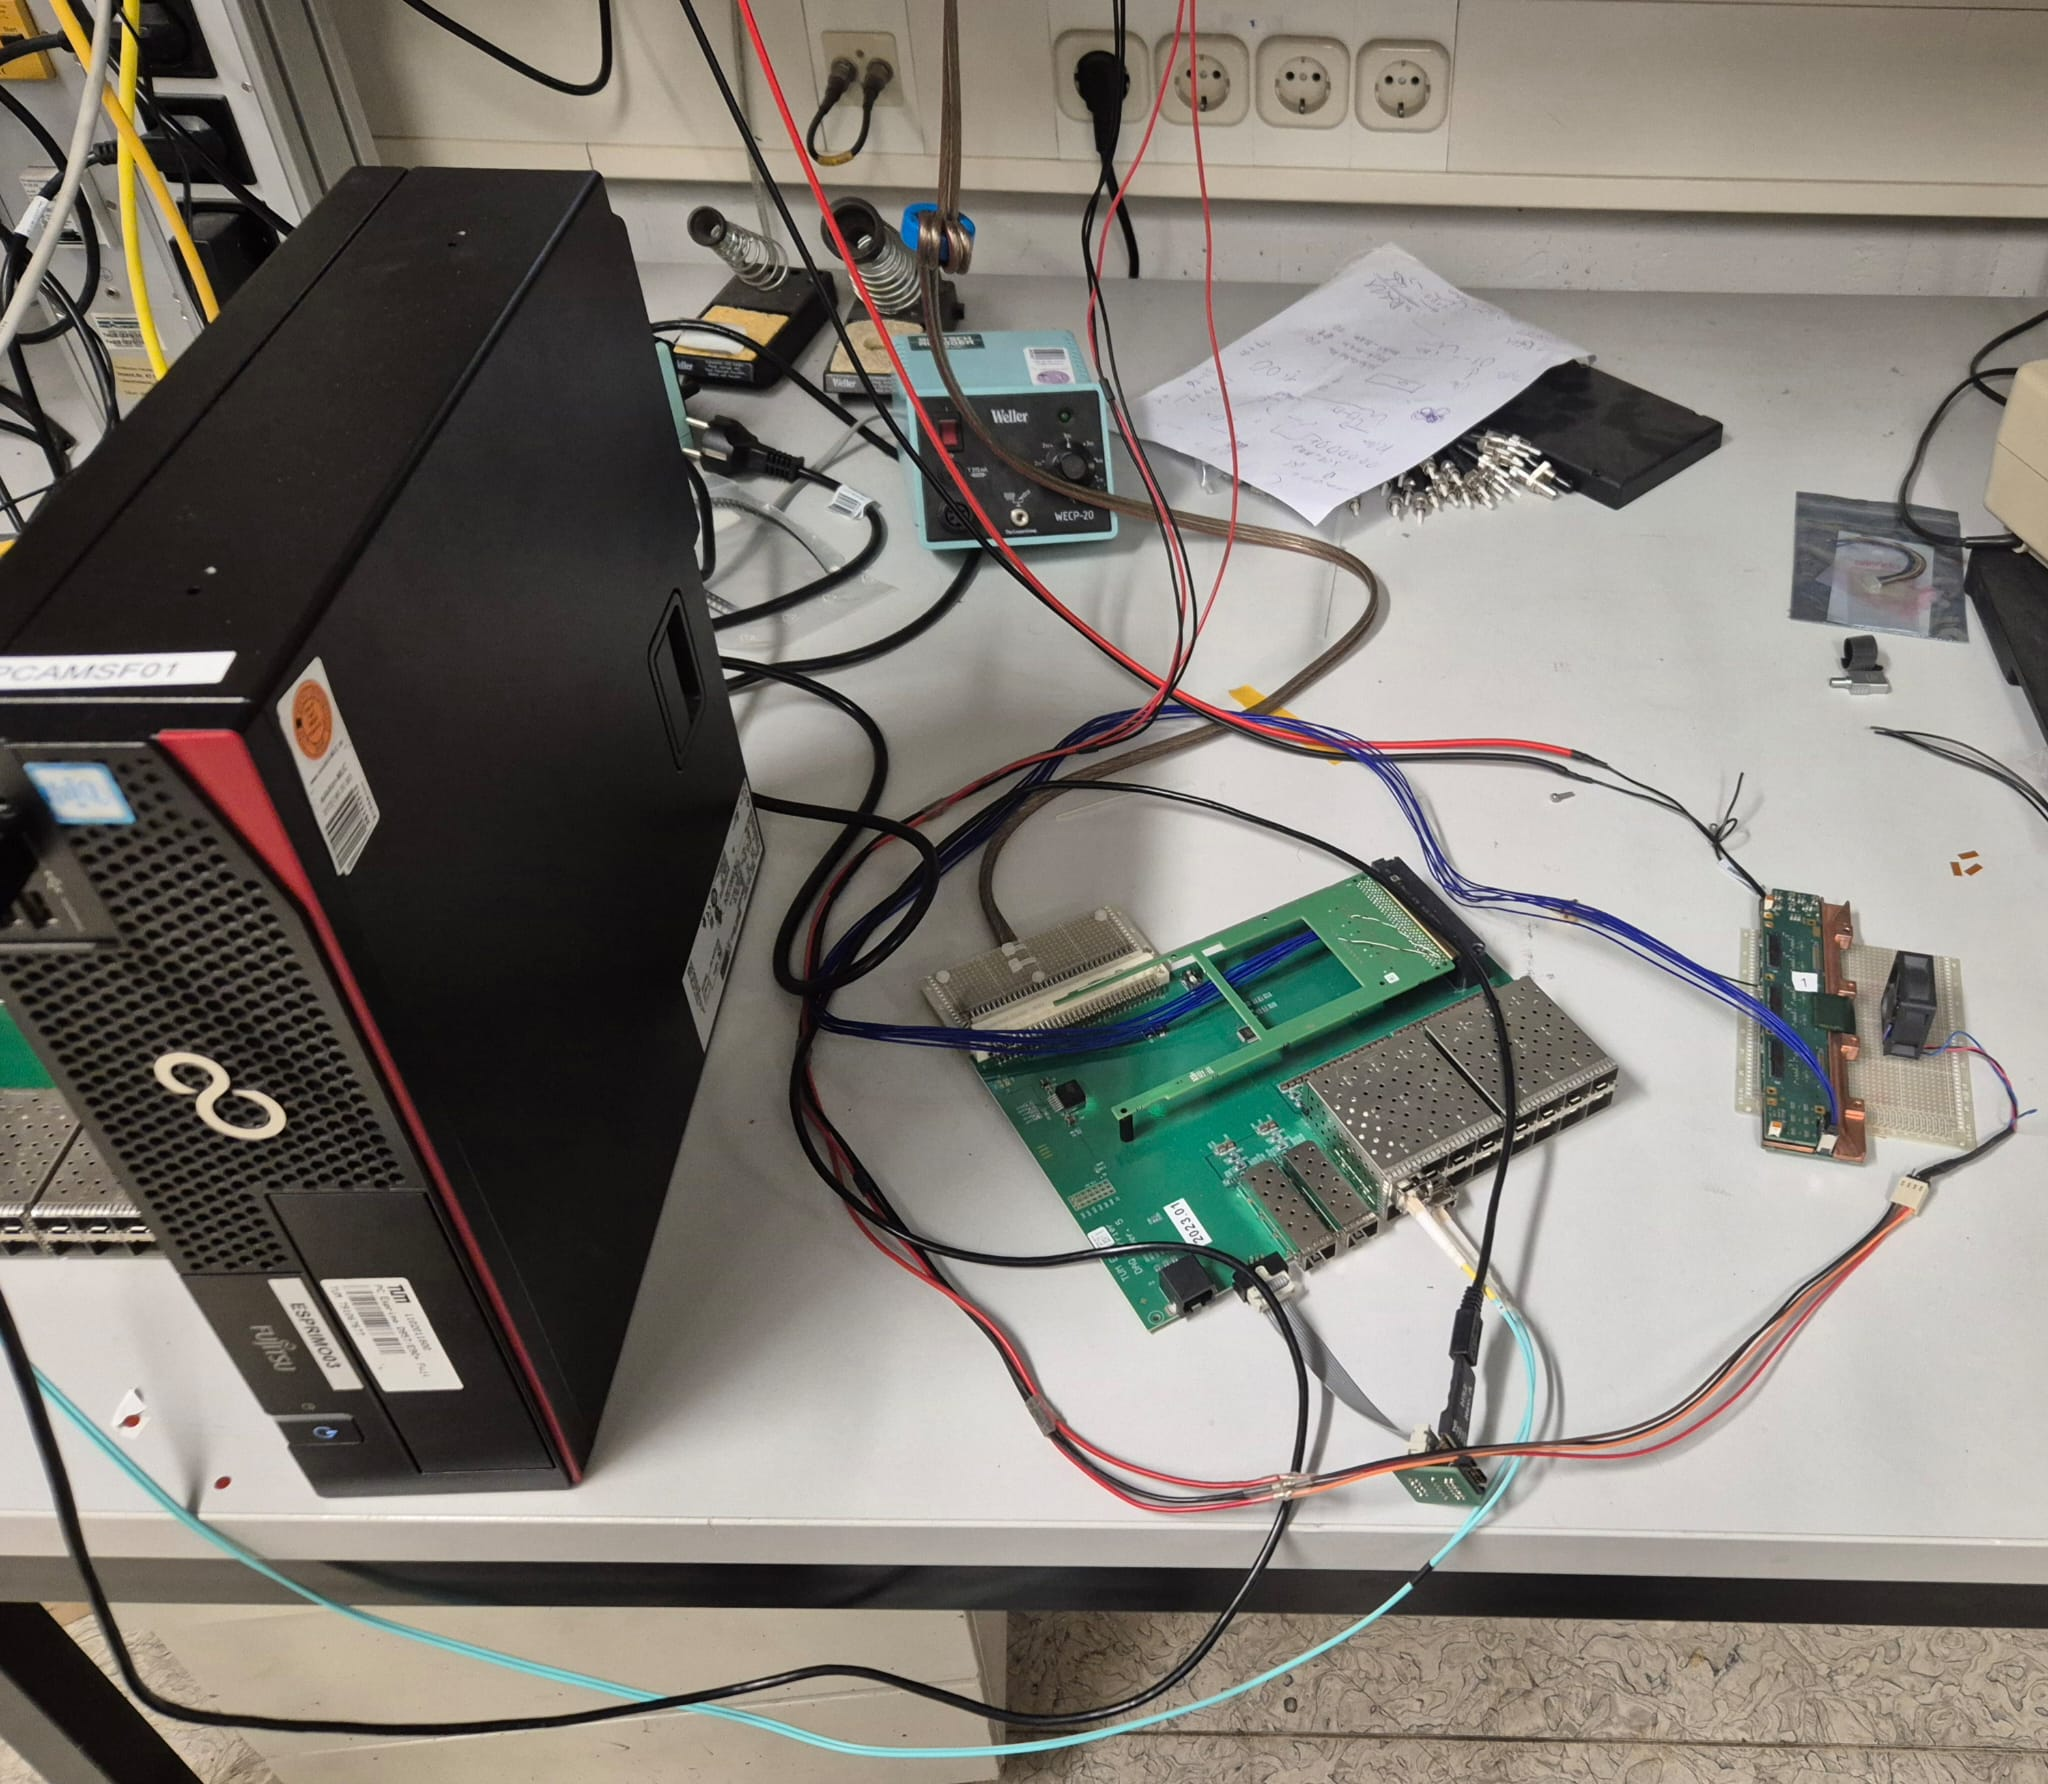
\includegraphics[width=0.8\textwidth]{WhatsApp Bild 2024-12-05 um 16.27.30_2637fa81.jpg}%{noise_setup.png}%{E18Logo.png}%
    \caption{Experimental setup for the threshold scan of the frontend electronics of the scintillating fiber hodoscope.}
    \label{fig:noise_setup}
\end{figure}
The scan will be performed by the controlling computer, 
which will scan through a range of thresholds of the time discriminator of the Citiroc1A ASIC and record the number of hits per second on each channel with an intergration time of \SI{400}{\milli\second}.
This scan will be preformed for several different high gains near the maximum value of 62.
\newline
For comparison, the threshold scan will also be performed with the same configuration of the Citiroc1A ASICs on a testboard provided by Weeroc, 
with the setup shown in Figure \ref{fig:noise_setup_testboard}.
\begin{figure}[H]
    \centering
    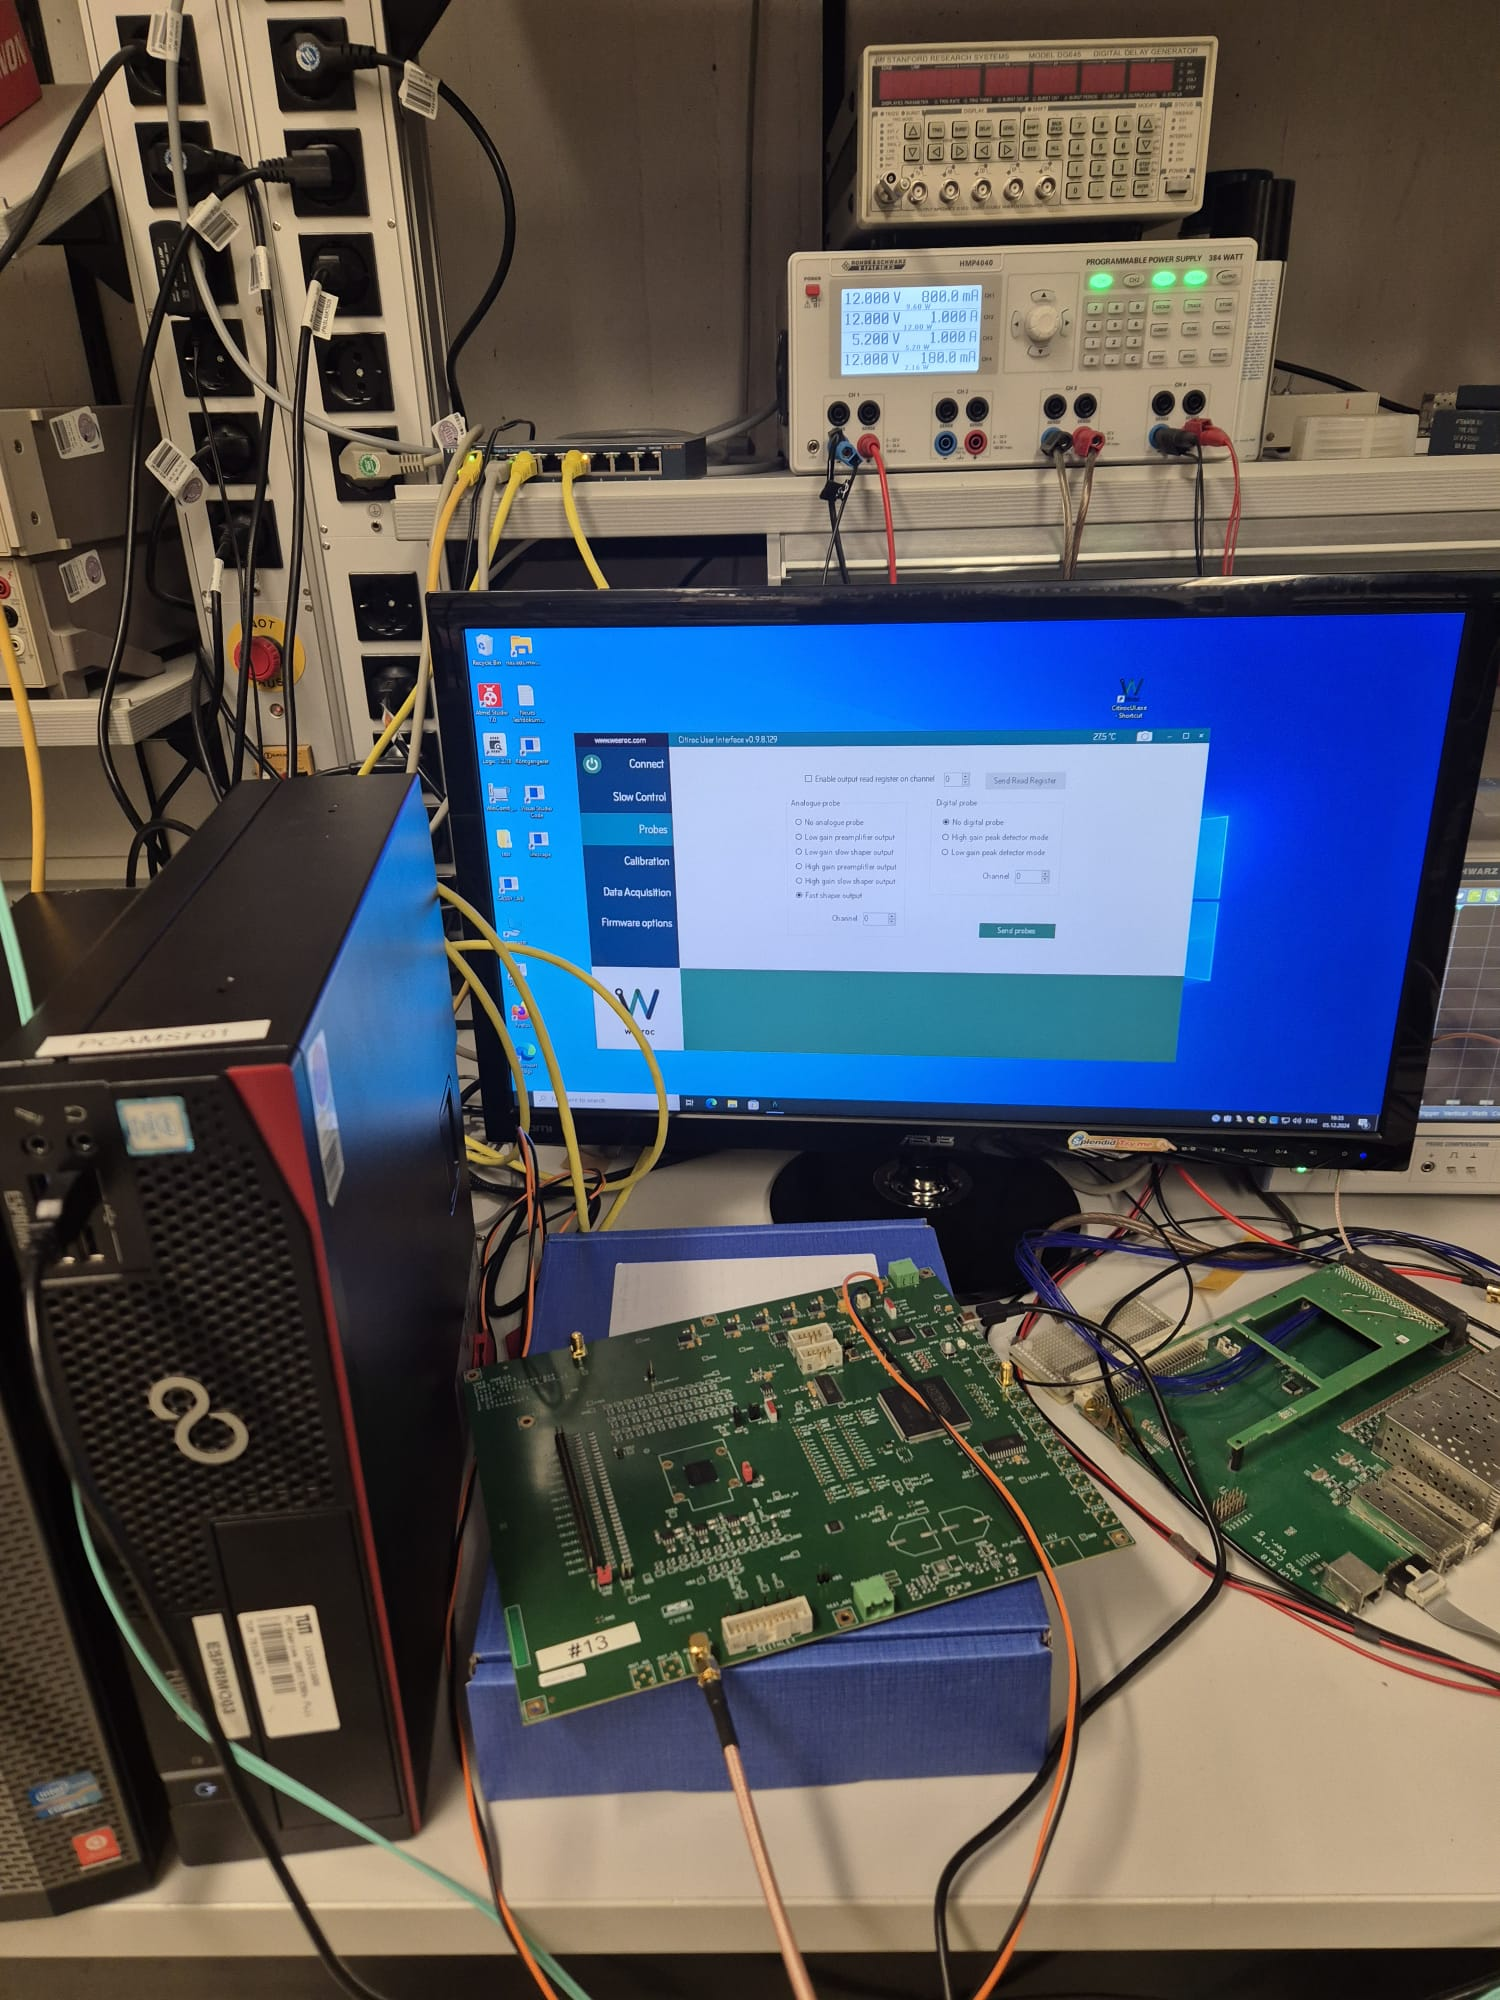
\includegraphics[width=0.8\textwidth]{WhatsApp Bild 2024-12-05 um 16.35.49_ef329d4e.jpg}%{noise_setup_testboard.png}%{E18Logo.png}%
    \caption{Experimental setup for the threshold scan with a testboard provided by Weeroc.}
    \label{fig:noise_setup_testboard}
\end{figure}

\subsection{Theoretical Backround for the Threshold Scan} \label{sec:noise_theory}
The noise on the unconnected frontend electronics is assumed to be of gaussian distribution,
\begin{equation}
    P(x) = \frac{1}{\sqrt{2\pi}\sigma}e^{-\frac{(x-\mu)^2}{2\sigma^2}}
\end{equation}
where $\mu$ is the mean and $\sigma$ the standard deviation of the noise.\autocite{Theorynoise}
\newline
The number of hits per second on each channel of the Citiroc1A ASIC is assumed to be proportional to the number of noise events above the threshold of the time discriminator, but limited by the maximal trigger rate of the fast shaper Citiroc1A ASICs
and thus only approximately proportional to the integral of the noise distribution above the threshold.\autocite{Theorynoise}
\newline
The number of hits per second vs the threshold of the time discriminator is expected to follow an S-curve, which can be described by a modified error function,
\begin{equation}
    N = \frac{A}{2} \left( 1 - \text{erf} \left( \frac{x - \mu}{\sqrt{2}\sigma} \right) \right)
\end{equation}
where $N$ is the number of hits per second, $x$ the threshold of the time discriminator and A an renormalization factor.\autocite{Theorynoise}